% !TEX root = ../main.tex

\chapter{Introduction}
\label{ch:introduction}

% \section{General Notation}
% First, I am defining the notation I used throughout this thesis. For the scalars, I used regular, normal-weight variables such as $x$. Vectors are represented by bold lower-case variables like $\mathbf{x}$. Tensors and matrices are denoted by bold upper-case characters, such as $\mathbf{X}$. In summary:
% \begin{align*}
% x&: \text{Scalar} \\
% \mathbf{x}&: \text{Vector} \\
% \mathbf{X}&: \text{Matrix or tensor}
% \end{align*}
% \todo[inline]{Useful? Everything covered?}

\section{Reinforcement Learning Control Problems}
Control problems appear in the context of both reinforcement learning and control theory. Thus, we often see vocabulary specific to control theory in the context of reinforcement learning. A control problem, generally explained, is a dynamic system described by state variables. The choice of controls or actions determines how the system will behave in the future. The goal of a control problem is to work out a strategy that causes the system to terminate in the desired target state. Reinforcement learning and approaches in control theory offer a framework to solve such control problems (\cite{bucsoniu2018reinforcement}). Even though the two fields embark on the same problem, the research communities remained mostly disjoint, leading to different approaches to the same problem. Reinforcement learning often makes model-free predictions from data, whereas control theory often defines well-specified models (\cite{recht2018tour}). In this thesis, I will focus on reinforcement learning frameworks to solve control problems.

Reinforcement learning is an area of machine learning that involves learning the optimal behavior to maximize a reward signal inside a dynamic environment. The learning process is marked by trial-and-error interactions with the environment. The learner does not know which actions lead to which rewards until he tries them (\cite{kaelbling1996reinforcement}).

Reinforcement learning differs from supervised learning, where learning is achieved through a training set with labeled examples. Each sample of the training data represents a description of the situation together with a label that marks how the system should react in that situation. The goal of the learning process is to generalize the optimal actions given a certain situation so that the system acts correctly in situations outside of the training set. In reinforcement learning, there are no labels available beforehand. In addition, we can also not classify reinforcement learning as unsupervised learning, where we typically try to find a hidden structure in a set of unlabeled data. With reinforcement learning, we do not try to find some structure in the data but solely try to maximize the reward signal. Therefore, alongside supervised learning, unsupervised learning, and maybe additional paradigms, reinforcement learning is considered to be a third machine learning paradigm. One additional challenge we do not see in the other branches of machine learning is the trade-off between \textit{exploration} and \textit{exploitation}. For a high reward, the reinforcement learning agent should take an action that it has tried in the past and was effective. It should therefore exploit the knowledge gained previously. However, to discover this beneficial action, it has to explore actions it has not taken before (\cite{sutton2018reinforcement}).

To overcome the mentioned difficulties unique to reinforcement learning, we need to experiment with alternative models and strategies than those used for supervised or unsupervised learning.

\todo[inline]{Include MDP.}


\section{Classic Reinforcement Learning}
In reinforcement learning, we have an agent and an environment. The agent can take on actions to interact with the environment. The environment, on the other hand, always holds a certain state that can be altered by the actions of the agent. The goal of the agent in classic reinforcement learning is to learn a policy $\pi$ that drives the system into the desired state by taking the right actions. For example, the goal might be to solve skill games like Ball-in-a-Cup or Kendama (\cite{kober2010imitation}). As mentioned before, we do not have labeled data beforehand as we do in supervised learning problems. We only get a scalar reward signal that indicates how well the agent performs. The goal of the agent is to maximize the cumulative rewards received by the environment. Therefore, the agent needs to learn optimal behavior only through trial-and-error interaction with the environment. This makes the problem structure much more challenging.
\begin{figure}[!ht]
\centering
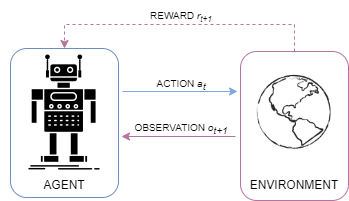
\includegraphics[width=.6\textwidth]{RL_agent_env}
\caption[Interaction loop between an RL agent and the environment]{
  \textbf{Interaction loop between an RL agent and the environment.}
  At timestep $t$, the agent receives the observation $o_t$ from the environment. The agent decides to select action $a_t$ and interacts with the environment. The enviornment changes and returns the next observation $o_{t+1}$ and the reward $r_{t+1}$ to the agent.
}
\label{fig:RL_agent_env}
\end{figure}
Figure~\ref{fig:RL_agent_env} illustrates the loop between the agent and the environment. The agent has received the observation $o_t$ from the environment and therefore knows the environment's current state. The agent then performs some action $a_t$ in the environment. The environment's state changes according to the received action and returns an observation $o_{t+1}$ indicating the current state of the environment and a reward $r_{t+1}$. One such interaction between the agent and the environment represents one \emph{timestep}.

The rewards correspond to an underlying reward function specific to the environment. The reward function is a function that maps the current state of the environment, the current action, and the subsequent state into a scalar value. It can be deterministic or can contain a random component making it stochastic. Depending on the problem, the reward can be sparse or dense. Sparse reward means that the reward function returns zero in most of its domain and only returns a meaningful reward in a few rare settings or at the end of the experiment. That introduces a immense challenge since we cannot know which particular actions led to success or failure. Optimization problems with this setting are generally challenging to solve. Dense reward environments return a meaningful reward at almost every time step, making the optimization process much easier.

Learning a policy that maximizes cumulative rewards is generally non-trivial. The agent can only learn through trial and error. If the policy is not explorative enough, we might get stuck in a local optimum and never reach the goal. However, if there is too much exploration we receive less reward. Thus, there needs to be a balance between exploration and exploitation. In addition, there is often a time delay for the reward. The consequence of an action might not be immediately visible to the agent. This problem is known as the credit-assignment problem in the literature (\cite{sutton2018reinforcement}).

We can solve reinforcement learning problems with methods based on value functions or methods based on policy search. The value function is a prediction of the future reward of landing in a specific state. It indicates how good or bad being in a certain state is. With methods based on value functions, the agent chooses the best action in the state. Methods based on policy search directly search for the optimal policy $\pi^*$ and do not need to maintain a value function model (\cite{8103164}).

As interest in neural networks and deep learning increased, deep reinforcement learning, which uses a neural network to estimate policies or value functions, attracted more attention.

\todo[inline]{Talk about sample efficiency? Include Q-Learning, reward shaping? show more the difference between this and dps}

\subsection{Neural Networks as Models}
\label{subsec:NN}
Neural networks are machine learning algorithms inspired by the functionalities of the human brain. They are applied successfully in many areas including in reinforcement learning problems. Neural networks consist of connected neurons or nodes that imitate the biological neurons of the brain sending signals to each other. A neuron receives one or multiple input values and calculates one or multiple output values. Figure [insert figure] illustrates one neuron. The neuron receives three input values and calculates one output value. For the caluclation of the ouptut, the neurons uses the assigned weights $w$. Thus, the output represents the sum of weighted inputs.

In a neural network, the neurons are arranged in connected layers. A network has at least an input and an output layer. We can further expand it with one or more hidden layers. Depending on the model, the connectivity between the layers differs. Figure~\ref{fig:neural_network_sketch} shows a sketch of a network with three hidden layers that are fully connected.
\begin{figure}[ht]
\centering
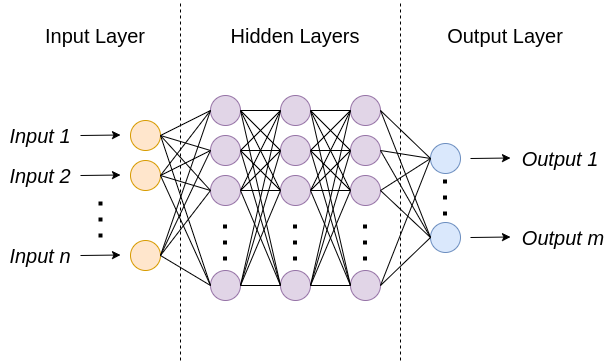
\includegraphics[width=.7\textwidth]{neural_network_sketch}
\caption[Sketch of a Neural Network]{
  \textbf{Sketch of a neural network.}
  The image shows a sketch of a neural network with three fully connected hidden layers. The network expects $n$ inputs and has $m$ possible outputs.
}
\label{fig:neural_network_sketch}
\end{figure}
Each neuron holds an associated weight and threshold. It receives an input and outputs the sum of weighted inputs. If this sum is greater than the associated threshold, the neuron gets activated.

A large part of the success of neural networks can be traced to the use of \textit{backpropagation}. Backpropagation uses information from the previous epoch (i.e. iteration) to adjust the weights of the network using the error gradient.

A neural network with one or more hidden layers defines a non-linear function. It is theoretically able to represent any function. Thus, neural networks are \textit{generic function approximators}. In addition, neural networks are highly expressive and flexible. In the context of reinforcement learning, they can be used to approximate a value function or a policy function. Deep reinforcement learning combines reinforcement learning with the methods from deep learning. It has been used in many applications including robotics, video games, and computer vision (\cite{franccois2018introduction}).

A sigmoid function is a mathematical function that maps an arbitrary input space into an output space with a small range, for example, 0 and 1. The function has a characteristic S-shaped curve. We can interpret the output space of the sigmoid function as a probability. The formula and a plot of the logistic sigmoid function in 2D are shown in Figure~\ref{fig:sigmoid}.
\begin{figure}[ht]
\centering
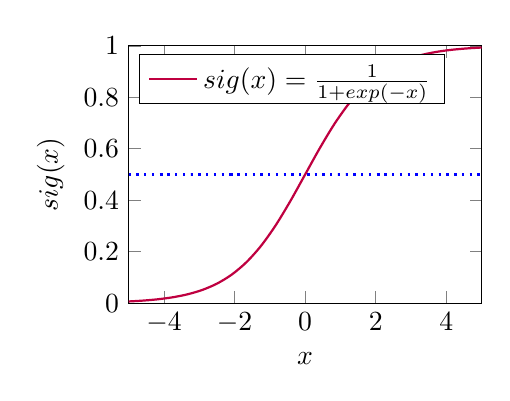
\begin{tikzpicture}
\begin{axis}[
      xmin = -5, xmax = 5,
      ymin = 0, ymax = 1,
      legend cell align = {left},
      legend pos = north west,
      width = 0.5\textwidth,
      height = 0.4\textwidth,
      xlabel = \(x\),
      ylabel = {\(sig(x)\)}
    ]
    \addplot[
        smooth,
        thick,
        purple
    ] {1 / (1 + exp(-x))};
    \addlegendentry{
    $sig(x) = \frac{1}{1 + exp(-x)}$
    }
    \addplot[
        smooth,
        thick,
        blue,
        dotted
    ] {0.5};
\end{axis}
\end{tikzpicture}
\caption[Sigmoid function]{
  \textbf{Sigmoid function.}
  The figure shows a plot of the logistic sigmoid function. The function maps an arbitrary input space into the range between 0 and 1. The output of the function can be interpreted as a probability. It is useful to scale data into a meaningful value.
}
\label{fig:sigmoid}
\end{figure}

The backpropagation algorithm's efficiency in calculating the gradient of an objective function is a key component of deep learning's success. However, there are certain limitations. For the backpropagation algorithm to be efficient, it relies on calculating accurate gradients. In fields like reinforcement learning, where we only have a reward signal that might be time delayed, this is a non-trivial task. In addition, there is a risk of getting stuck in a local optimum (\cite{ha2017visual}). These limits raise the question of which alternative models or techniques could be used that overcome these difficulties.


%However, neural networks also come with a few limitations or disadvantages. The backpropagation algorithm requires the calculation of an accurate gradient. Depending on the problem, this can be a challenging task. For example, calculating an accurate gradient in RL problems is usually non-trivial. Furthermore, there is a lack of understanding. The output of a neural network is often incomprehensible because of its complex structure.

\todo[inline]{Should NN be explained in more detail? Write more about DRL, include recent results, advantages, disadvantages. Improve transition to DRL and Sigmoid.}

\section{OpenAI Gym}
\label{sec:gym}
The research community requires high-quality benchmarks to compare algorithms and models applied to problems in reinforcement learning. There were already a few released benchmarks like the Arcade Learning Environment (\cite{bellemare2013arcade}) or the RLLab benchmark for continuous control (\cite{duan2016benchmarking}). OpenAI Gym\footnote{https://www.gymlibrary.ml/} combined the elements of these existing benchmarks in one toolkit. It provides a collection of tasks (called \textit{environments}) with varying levels of difficulties and challenges. The interface is the same for all environments, which makes it convenient to use. The environments represent general reinforcement learning problems, including control problems, that are widely used in the literature to compare different approaches. To interact with an environment, we first have to initialize it. We can do this with the predefined function \verb|make()|. The following Python code shows the initialization of the environment \verb|CartPole|:
\begin{minted}[linenos, frame=single]{python}
import gym
env = gym.make("CartPole-v0")
\end{minted}
As we are in the setting of reinforcement learning, we assume that an agent is acting inside the dynamic environment. In each step, the agent can take some action and receives a reward and a new observation in return from the environment. Both the action and observation space are predefined by the environment. In practice, an agent returns an action \verb|a0| with which we call the function \verb|step()| of the environment. The next code snippet shows an example of this behavior:
\begin{minted}[linenos, frame=single]{python}
observation, reward, done, info = env.step(a0)
\end{minted}
The observation and reward returned by the environment applies to the current time step. OpenAI Gym focuses on episodic reinforcement learning, where the agent acts in a series of episodes with a fixed length. The initial state of the environment in each episode is sampled randomly. An episode ends when certain termination criteria are met. For example, when the task is solved or when we max out on timesteps (\cite{1606.01540}).


\todo[inline]{Explain more, compare with Section~\ref{sec:environments} to not repeat}

\section{Direct Policy Search}
mention it as an alternative to Deep RL, mention it uses networks to approximate policy rather than value function \\ \\
Although using value functions to solve reinforcement learning problems has worked well in many applications, there are limitations. If the state space is not entirely observable, convergence problems can arise (\cite{el2005direct}). Additionally, in traditional value-based methods like Q-learning or temporal difference learning, the value function is computed iteratively with the help of bootstrapping. That often results in a bias in the quality assessment of state-action pairs for continuous state spaces. Another disadvantage of these methods is that the value functions are often discontinuous (\cite{deisenroth2013survey}).

Studies suggest that directly approximating a policy can be easier and delivers better results (\cite{sutton1999policy}; \cite{anderson2000approximating}). This alternative method to methods based on value functions is called \textit{direct policy search}. With direct policy search, the algorithm directly searches in the search space of policy representations discarding any value function (\cite{wierstra2010study}). Instead of approximating a value function, we approximate the policy directly with an independent function approximator. Thus, we directly approximate the action-state mapping.

\todo[inline]{Explain more, go more into advantages, find more papers with comparison}

\section{Neuroevolution}
special case of DPS: NN as policy approximator, train with evo \\ \\
Neuroevolution is a method that we can use for direct policy search. Like deep reinforcement learning, we employ a neural network as our model. In deep reinforcement learning, we typically use gradient-based learning strategies, whereas, in neuroevolution, we employ evolutionary algorithms to optimize the network parameters. That reduces the risk of being unable to estimate accurate gradients or being stuck in a local optimum. Evolutionary algorithms only require a measure of the network's performance, making them directly applicable for reinforcement learning problems. Thus, we can use it more widely in a variety of problem classes. \cite{such2017deep} showed that genetic algorithms, a subgroup of evolutionary algorithms, work well for the parameter search of neural networks. Even in hard reinforcement learning settings, including Atari and humanoid locomotion, they were able to achieve results at the scale of traditional deep reinforcement learning frameworks.

\todo[inline]{Explain more. more with direct policy search}

\section{Black-Box Optimization}
but what is evo? here's a primer on black box optimization \\ \\
In Black-Box Optimization (BBO), the problem structure, as well as the model, remains unknown. BBO methods optimize a parametrization without any constraints on the problem, model or solution needed. Thus, there is no constraint on differentiability or convexity. The optimization is done solely based on a score or cumulative reward, which makes these methods directly applicable to reinforcement learning problems.
\todo[inline]{Explain more}

\subsection{Random Weight Guessing}
Randomization and RWG (uniform distribution) \\ \\
Random Weight Guessing (RWG) is the simplest BBO method. With RWG, we repeatedly randomly initialize the weights of a model until the resulting model classifies all training instances correctly. Then we test the model on a separate test set (\cite{schmidhuber2001evaluating}). RWG is not a reasonable learning algorithm, but it can be used as an analysis method (\cite{oller_analyzing_2020}).
\todo[inline]{Explain more, include limitations (expensive algorithms)}

\subsection{Evolution Strategies}
ES-(1+1) (normal, adapt mean) \\ \\
Evolution Strategies (ES) belong to the class of evolutionary algorithms and are best suited for continuous optimization. They are directly inspired by the idea of evolution in nature and use the concept of mutation and selection. ES are implemented in a loop where one iteration is called a generation. In each generation new individuals (candidate solutions) are generated using the current parents. We continue with the next generation until a stopping criteria is met. ES are multi-agent algorithms which means that they generate multiple parametrizations that explore a different path or area in the optimization space independently. This exploration prevents us from landing in a local optimum.

\textbf{(1 + 1)-ES:} The population model (1 + 1) means that we maintain only one individual. For the next generation, we generate one new offspring as a variation of the parent, drawn from the normal distribution. For this, we adapt the mean of the distribution according to the parent. Then we keep either the parent or the child based on which performed had a better fitness score. Algorithm~\ref{alg:ES} shows this process in pseudocode.
\begin{algorithm}
\caption{(1 + 1)-ES in $d$ dimensions}
\begin{algorithmic}[1]
\State Parameter: $\sigma > 0$
\State Initialization: $x = x_0 \in \mathbb{R}^d$
\While{not done}
    \State Sample $x' \sim \mathcal{N}(x, \sigma^2 I)$
    \If{$f(x') \leq f(x)$}
      \State $x \leftarrow x'$
    \EndIf
\EndWhile
\State Return $x$
\end{algorithmic}
\label{alg:ES}
\end{algorithm}

\todo[inline]{Explain more}


\subsection{Covariance Matrix Adaptation Evolution Strategy}
CMA-ES (which is a ES-(mu,lambda)) (normal, adapt mean, adapt covariance, large pop) \\ \\
Covariance Matrix Adaptation Evolution Strategy (CMA-ES) is a method for non-linear, non-convex optimization problems in continuous domain. For each iteration (generation), a population of new individuals is generated by sampling a multivariate normal distribution. After each iteration, the mean and the covariance matrix is updated (\cite{hansen2016cma}).

\todo[inline]{Include formulas from tutorial}

\subsection{Function Approximators}
With BBO, we can use any function approximator.

\section{Research Questions}
\label{sec:research_questions}
Start from the experiments. They are your answer. Which question do they answer? These are your research questions. \\
In the experiments section, mention explicitly which question each answers \\ \\
The main goal of this thesis is to compare alternative models to neural networks. To analyze and compare the different models and their architectures, I formulated the following research questions:
\begin{enumerate}
  \item How do function approximators other than neural networks compare with the latter?
  \item What advantages and disadvantages can we see with other function approximators?
  \item What impact has the bias on the performance of the model?
  % \begin{enumerate}
  %   \item Does increasing the number of weights worsen the performance of the model?
  %   \item Does a neural network with more than two hidden layers yield worse scores?
  %   \item Does the neural network's performance suffer from an increase in the number of neurons?
  %   \item Does the difficulty of the environment affect the observed effect of the bias?
  % \end{enumerate}
\end{enumerate}

\todo[inline]{Work on questions.}
